\chapter{Discrete and censored dependent variables}
\label{chap:discr-models}

This chapter deals with models for dependent variables that are
discrete or censored or otherwise limited (as in event counts or
durations, which must be positive) and that therefore call for
estimation methods other than the classical linear model. We discuss
several estimators (mostly based on the Maximum Likelihood principle),
adding some details and examples to complement the material on
these methods in the \emph{Gretl Command Reference}.

\section{Logit and probit models}
\label{sec:logit-probit}

It often happens that one wants to specify and estimate a model in
which the dependent variable is not continuous, but discrete. A
typical example is a model in which the dependent variable is the
occupational status of an individual (1 = employed, 0 = unemployed). A
convenient way of formalizing this situation is to consider the
variable $y_i$ as a Bernoulli random variable and analyze its
distribution conditional on the explanatory variables $x_i$.  That is,
%
\begin{equation}
  \label{eq:qr-Bernoulli}
  y_i = \left\{ 
    \begin{array}{ll} 
      1 & P_i \\ 0 & 1 - P_i 
    \end{array}
    \right.
\end{equation}
%
where $P_i = P(y_i = 1 | x_i) $ is a given function of the explanatory
variables $x_i$.

In most cases, the function $P_i$ is a cumulative distribution
function $F$, applied to a linear combination of the $x_i$s. In the
probit model, the normal cdf is used, while the logit model employs
the logistic function $\Lambda()$. Therefore, we have
%
\begin{eqnarray}
  \label{eq:qr-link}
  \textrm{probit} & \qquad & P_i = F(z_i) = \Phi(z_i)  \\
  \textrm{logit}  & \qquad & P_i = F(z_i) = \Lambda(z_i) = \frac{1}{1 + e^{-z_i}} \\
  & &z_i = \sum_{j=1}^k x_{ij} \beta_j
\end{eqnarray}
%
where $z_i$ is commonly known as the \emph{index} function. Note that
in this case the coefficients $\beta_j$ cannot be interpreted as the
partial derivatives of $E(y_i | x_i)$ with respect to
$x_{ij}$.  However, for a given value of $x_i$ it is possible to
compute the vector of ``slopes'', that is
\[
  \mathrm{slope}_j(\bar{x}) = \left. \pder{F(z)}{x_j} \right|_{z =
    \bar{z}}
\]
\app{Gretl} automatically computes the slopes, setting each
explanatory variable at its sample mean.

Another, equivalent way of thinking about this model is in terms of
an unobserved variable $y^*_i$ which can be described thus:
%
\begin{equation}
  \label{eq:qr-latent}
  y^*_i = \sum_{j=1}^k x_{ij} \beta_j + \varepsilon_i = z_i  +
  \varepsilon_i 
\end{equation}
%
We observe $y_i = 1$ whenever $y^*_i > 0$ and $y_i = 0$ otherwise. If
$\varepsilon_i$ is assumed to be normal, then we have the probit
model. The logit model arises if we assume that the density function
of $\varepsilon_i$ is
%
\[
  \lambda(\varepsilon_i) =
  \pder{\Lambda(\varepsilon_i)}{\varepsilon_i} =
  \frac{e^{-\varepsilon_i}}{(1 + e^{-\varepsilon_i})^2}
\]

Both the probit and logit model are estimated in \app{gretl} via
maximum likelihood, where the log-likelihood can be written as
\begin{equation}
  \label{eq:qr-loglik}
  L(\beta) = \sum_{y_i=0} \ln [ 1 - F(z_i)] + \sum_{y_i=1} \ln F(z_i),
\end{equation}
which is always negative, since $0 < F(\cdot) < 1$.  Since the score
equations do not have a closed form solution, numerical optimization
is used. However, in most cases this is totally transparent to the
user, since usually only a few iterations are needed to ensure
convergence. The \option{verbose} switch can be used to track the
maximization algorithm.

\begin{script}[htbp]
  \caption{Estimation of simple logit and probit models}
  \label{simple-QR}
\begin{scode}
open greene19_1

logit GRADE const GPA TUCE PSI
probit GRADE const GPA TUCE PSI
\end{scode}
\end{script}

As an example, we reproduce the results given in chapter 21 of
\cite{greene00}, where the effectiveness of a program for teaching
economics is evaluated by the improvements of students' grades.
Running the code in example \ref{simple-QR} gives the following
output:
\begin{code}

Model 1: Logit estimates using the 32 observations 1-32
Dependent variable: GRADE

      VARIABLE       COEFFICIENT        STDERROR      T STAT       SLOPE
                                                                  (at mean)
  const               -13.0213           4.93132      -2.641
  GPA                   2.82611          1.26294       2.238      0.533859   
  TUCE                  0.0951577        0.141554      0.672      0.0179755  
  PSI                   2.37869          1.06456       2.234      0.449339   

  Mean of GRADE = 0.344
  Number of cases 'correctly predicted' = 26 (81.2%)
  f(beta'x) at mean of independent vars = 0.189
  McFadden's pseudo-R-squared = 0.374038
  Log-likelihood = -12.8896
  Likelihood ratio test: Chi-square(3) = 15.4042 (p-value 0.001502)
  Akaike information criterion (AIC) = 33.7793
  Schwarz Bayesian criterion (BIC) = 39.6422
  Hannan-Quinn criterion (HQC) = 35.7227

           Predicted
             0    1
  Actual 0  18    3
         1   3    8

Model 2: Probit estimates using the 32 observations 1-32
Dependent variable: GRADE

      VARIABLE       COEFFICIENT        STDERROR      T STAT       SLOPE
                                                                  (at mean)
  const                -7.45232          2.54247      -2.931
  GPA                   1.62581          0.693883      2.343      0.533347   
  TUCE                  0.0517288        0.0838903     0.617      0.0169697  
  PSI                   1.42633          0.595038      2.397      0.467908   

  Mean of GRADE = 0.344
  Number of cases 'correctly predicted' = 26 (81.2%)
  f(beta'x) at mean of independent vars = 0.328
  McFadden's pseudo-R-squared = 0.377478
  Log-likelihood = -12.8188
  Likelihood ratio test: Chi-square(3) = 15.5459 (p-value 0.001405)
  Akaike information criterion (AIC) = 33.6376
  Schwarz Bayesian criterion (BIC) = 39.5006
  Hannan-Quinn criterion (HQC) = 35.581

           Predicted
             0    1
  Actual 0  18    3
         1   3    8

\end{code}

In this context, the \dollar{uhat} accessor function takes a special
meaning: it returns generalized residuals as defined in
\citet*{gourieroux87}, which can be interpreted as unbiased estimators
of the latent disturbances $\varepsilon_i$. These are defined as
%
\begin{equation}
  \label{eq:QR-genres}
  u_i = \left\{
    \begin{array}{ll}
      y_i - \hat{P}_i & \textrm{for the logit model} \\
      y_i\cdot \frac{\phi(\hat{z}_i)}{\Phi(\hat{z}_i)} - 
      ( 1 - y_i ) \cdot \frac{\phi(\hat{z}_i)}{1 - \Phi(\hat{z}_i)}
      & \textrm{for the probit model} \\
    \end{array}
    \right.
\end{equation}

Among other uses, generalized residuals are often used for diagnostic
purposes.  For example, it is very easy to set up an omitted variables
test equivalent to the familiar LM test in the context of a linear
regression; example \ref{QR-add} shows how to perform a variable
addition test.

\begin{script}[htbp]
  \caption{Variable addition test in a probit model}
  \label{QR-add}
\begin{scode}
open greene19_1

probit GRADE const GPA PSI
series u = $uhat 
%$
ols u const GPA PSI TUCE -q
printf "Variable addition test for TUCE:\n"
printf "Rsq * T = %g (p. val. = %g)\n", $trsq, pvalue(X,1,$trsq) 
\end{scode}
\end{script}

\subsection{The perfect prediction problem}
\label{sec:perfpred}

One curious characteristic of logit and probit models is that (quite
paradoxically) estimation is not feasible if a model fits the data
perfectly; this is called the \emph{perfect prediction problem}. The
reason why this problem arises is easy to see by considering equation
(\ref{eq:qr-loglik}): if for some vector $\beta$ and scalar $k$ it's
the case that $z_i < k$ whenever $y_i=0$ and $z_i > k$ whenever
$y_i=1$, the same thing is true for any multiple of $\beta$. Hence,
$L(\beta)$ can be made arbitrarily close to 0 simply by choosing
enormous values for $\beta$. As a consequence, the log-likelihood has
no maximum, despite being bounded.

\app{Gretl} has a mechanism for preventing the algorithm from
iterating endlessly in search of a non-existent maximum. One sub-case
of interest is when the perfect prediction problem arises because of
a single binary explanatory variable. In this case, the offending
variable is dropped from the model and estimation proceeds with the
reduced specification. Nevertheless, it may happen that no single
``perfect classifier'' exists among the regressors, in which case
estimation is simply impossible and the algorithm stops with an
error. This behavior is triggered during the iteration process if
\[
  \stackunder{i: y_i = 0}{\max z_i} \, < \,
  \stackunder{i: y_i = 1}{\min z_i}  
\]
If this happens, unless your model is trivially mis-specified (like
predicting if a country is an oil exporter on the basis of oil
revenues), it is normally a small-sample problem: you probably just
don't have enough data to estimate your model. You may want to drop
some of your explanatory variables.

This problem is well analyzed in \cite{stokes04}; the results therein
are replicated in the example script \texttt{murder\_rates.inp}. 

\section{Ordered response models}
\label{sec:ordered}

These models constitute a simple variation on ordinary logit/probit
models, and are usually applied when the dependent variable is a
discrete and ordered measurement --- not simply binary, but on an
ordinal rather than an interval scale.  For example, this sort of
model may be applied when the dependent variable is a qualitative
assessment such as ``Good'', ``Average'' and ``Bad''.  

In the general case, consider an ordered response variable, $y$, that
can take on any of the $J+1$ values ${0,1,2,\dots,J}$.  We suppose, as
before, that underlying the observed response is a latent variable,
\[
  y^* = X\beta + \varepsilon = z + \varepsilon
\]
Now define ``cut points'', $\alpha_1 < \alpha_2 < \cdots < \alpha_J$,
such that
%
\begin{equation*}
  \begin{array}{ll}
    y = 0 & \textrm{if } \, y^* \leq \alpha_1 \\
    y = 1 & \textrm{if } \, \alpha_1 < y^* \leq \alpha_2 \\
    \vdots \\
    y = J & \textrm{if } \, y^* > \alpha_J \\
  \end{array}
\end{equation*}
For example, if the response takes on three values there will be two
such cut points, $\alpha_1$ and $\alpha_2$. 

The probability that individual $i$ exhibits response $j$, conditional
on the characteristics $x_i$, is then given by
%
\begin{equation}
  \label{eq:QR-ordered}
  P(y_i = j \,|\, x_i) = \left\{
    \begin{array}{ll}
      P(y^* \leq \alpha_1 \,|\, x_i) = F(\alpha_1 - z_i) & \textrm{for }\, j = 0 \\
      P(\alpha_j < y^* \leq \alpha_{j+1} \,|\, x_i) = 
      F(\alpha_{j+1} - z_i) -  F(\alpha_j - z_i) & \textrm{for }\, 0 < j < J \\
      P(y^* > \alpha_J \,|\, x_i) = 1 -  F(\alpha_J - z_i) & \textrm{for }\, j = J 
    \end{array}
    \right.
\end{equation}
%
The unknown parameters $\alpha_j$ are estimated jointly with the
$\beta$s via maximum likelihood.  The $\hat{\alpha}_j$ estimates are
reported by \app{gretl} as \texttt{cut1}, \texttt{cut2} and so on.

In order to apply these models in \app{gretl}, the dependent variable
must either take on only non-negative integer values, or be explicitly
marked as discrete.  (In case the variable has non-integer values, it
will be recoded internally.)  Note that \app{gretl} does not provide a
separate command for ordered models: the \texttt{logit} and
\texttt{probit} commands automatically estimate the ordered version if
the dependent variable is acceptable, but not binary.

Note that the $\alpha_j$ parameters can be shifted arbitrarily by
adding a constant to $z_i$, so the model is under-identified if there
is some linear combination of the explanatory variables which is
constant. The most obvious case in which this occurs is when the model
contains a constant term; for this reason, \app{gretl} drops
automatically the intercept if present. However, it may happen that
the user inadventently specifies a list of regressors that may be
combined in such a way to produce a constant (for example, by using a
full set of dummy variables for a discrete factor). If this happens,
\app{gretl} will also drop any offending regressors.

\begin{script}[htbp]
  \caption{Ordered probit model}
  \label{ex:oprobit}
\begin{scode}
/*
  Replicate the results in Wooldridge, Econometric Analysis of Cross
  Section and Panel Data, section 15.10, using pension-plan data from
  Papke (AER, 1998).

  The dependent variable, pctstck (percent stocks), codes the asset
  allocation responses of "mostly bonds", "mixed" and "mostly stocks"
  as {0, 50, 100}.

  The independent variable of interest is "choice", a dummy indicating
  whether individuals are able to choose their own asset allocations.
*/

open pension.gdt

# demographic characteristics of participant
list DEMOG = age educ female black married
# dummies coding for income level
list INCOME = finc25 finc35 finc50 finc75 finc100 finc101

# Papke's OLS approach
ols pctstck const choice DEMOG INCOME wealth89 prftshr
# save the OLS choice coefficient 
choice_ols = $coeff(choice)

# estimate ordered probit
probit pctstck choice DEMOG INCOME wealth89 prftshr

k = $ncoeff
matrix b = $coeff[1:k-2]
a1 = $coeff[k-1]
a2 = $coeff[k]

/* 
   Wooldridge illustrates the 'choice' effect in the ordered probit 
   by reference to a single, non-black male aged 60, with 13.5 years 
   of education, income in the range $50K - $75K and wealth of $200K, 
   participating in a plan with profit sharing.
*/
matrix X = {60, 13.5, 0, 0, 0, 0, 0, 0, 1, 0, 0, 200, 1}

# with 'choice' = 0
scalar Xb = (0 ~ X) * b
P0 = cdf(N, a1 - Xb)
P50 = cdf(N, a2 - Xb) - P0
P100 = 1 - cdf(N, a2 - Xb)
E0 = 50 * P50 + 100 * P100

# with 'choice' = 1
Xb = (1 ~ X) * b
P0 = cdf(N, a1 - Xb)
P50 = cdf(N, a2 - Xb) - P0
P100 = 1 - cdf(N, a2 - Xb)
E1 = 50 * P50 + 100 * P100

printf "\nWith choice, E(y) = %.2f, without E(y) = %.2f\n", E1, E0
printf "Estimated choice effect via ML = %.2f (OLS = %.2f)\n", E1 - E0,
  choice_ols
\end{scode}
\end{script}

Example \ref{ex:oprobit} reproduces the results presented in section
15.10 of \cite{wooldridge-panel}.  The question of interest in this
analysis is what difference it makes, to the allocation of assets
in pension funds, whether individual plan participants have a
choice in the matter.  The response variable is an ordinal measure of
the weight of stocks in the pension portfolio.  Having reported the
results of estimation of the ordered model, Wooldridge illustrates the
effect of the \texttt{choice} variable by reference to an ``average''
participant.  The example script shows how one can compute this effect
in \app{gretl}.  

After estimating ordered models, the \dollar{uhat} accessor yields
generalized residuals as in binary models; additionally, the
\dollar{yhat} accessor function returns $\hat{z}_i$, so it is
possible to compute an unbiased estimator of the latent variable
$y^*_i$ simply by adding the two together.

\section{Multinomial logit}
\label{sec:mlogit}

When the dependent variable is not binary and does not have a natural
ordering, \emph{multinomial} models are used.  Multinomial logit is
supported in \app{gretl} via the \verb|--multinomial| option to the
\texttt{logit} command.  Simple models can also be handled via the
\texttt{mle} command (see chapter \ref{chap:mle}). We give here an
example of such a model.  Let the dependent variable, $y_i$, take on
integer values $0,1,\dots p$.  The probability that $y_i = k$ is given
by
\[
  P(y_i = k |  x_i) = \frac{\exp(x_i \beta_k)}{\sum_{j=0}^p \exp(x_i \beta_j)}
\]
For the purpose of identification one of the outcomes must be taken as
the ``baseline''; it is usually assumed that $\beta_0 = 0$, in which case
\[
  P(y_i = k |  x_i) = \frac{\exp(x_i \beta_k)}{1 + \sum_{j=1}^p \exp(x_i \beta_j)} 
\]
and
\[
  P(y_i = 0 |  x_i) = \frac{1}{1 + \sum_{j=1}^p \exp(x_i \beta_j)} .
\]

\begin{script}[htbp]
  \caption{Multinomial logit}
  \label{ex:mlogit}
Input:
\begin{scodebit}
open keane.gdt
smpl (year=87) --restrict
logit status 0 educ exper expersq black --multinomial
\end{scodebit}
Output (selected portions):
\begin{scodebit}
Model 1: Multinomial Logit, using observations 1-1738 (n = 1717)
Missing or incomplete observations dropped: 21
Dependent variable: status
Standard errors based on Hessian

             coefficient   std. error      z      p-value 
  --------------------------------------------------------
  status = 2
  const      10.2779       1.13334       9.069    1.20e-19 ***
  educ       -0.673631     0.0698999    -9.637    5.57e-22 ***
  exper      -0.106215     0.173282     -0.6130   0.5399  
  expersq    -0.0125152    0.0252291    -0.4961   0.6199  
  black       0.813017     0.302723      2.686    0.0072   ***
  status = 3
  const       5.54380      1.08641       5.103    3.35e-07 ***
  educ       -0.314657     0.0651096    -4.833    1.35e-06 ***
  exper       0.848737     0.156986      5.406    6.43e-08 ***
  expersq    -0.0773003    0.0229217    -3.372    0.0007   ***
  black       0.311361     0.281534      1.106    0.2687  

Mean dependent var   2.691322   S.D. dependent var   0.573502
Log-likelihood      -907.8572   Akaike criterion     1835.714
Schwarz criterion    1890.198   Hannan-Quinn         1855.874

Number of cases 'correctly predicted' = 1366 (79.6%)
Likelihood ratio test: Chi-square(8) = 583.722 [0.0000]  
\end{scodebit}
\end{script}

Example~\ref{ex:mlogit} reproduces Table 15.2 in
\cite{wooldridge-panel}, based on data on career choice from
\cite{keane97}.  The dependent variable is the occupational status of
an individual (0 = in school; 1 = not in school and not working; 2 =
working), and the explanatory variables are education and work
experience (linear and square) plus a ``black'' binary variable.  The
full data set is a panel; here the analysis is confined to a
cross-section for 1987. 

\section{Bivariate probit}
\label{sec:biprobit}

The bivariate probit model is simply a two-equation system in which
each equation is a probit model, but the two disturbance terms may not
be independent. In formulae,
\begin{eqnarray}
  y^*_{1,i} = \sum_{j=1}^{k_1} x_{ij} \beta_j + \varepsilon_{1,i}  & \qquad &
  y_{1,i}=1  \Longleftrightarrow y^*_{1,i}>0 \\
  y^*_{2,i} = \sum_{j=1}^{k_2} z_{ij} \gamma_j + \varepsilon_{2,i} & \qquad &
  y_{2,i}=1  \Longleftrightarrow y^*_{2,i}>0 \\
  \left[ \begin{array}{c}
      \varepsilon_{2,i} \\ \varepsilon_{2,i}
    \end{array} \right] \sim 
  N \left[ 0, \left( \begin{array}{cc}
      1 & \rho \\ \rho & 1
    \end{array} \right) \right] 
\end{eqnarray}

\begin{itemize}
\item The explanatory variables for the first equation $x$ and for the
  second equation $z$ may overlap
\item example contained in \texttt{biprobit.inp}
\item \dollar{uhat} and \dollar{yhat} are matrices
\end{itemize}

FIXME: expand.


\section{The Tobit model}
\label{sec:tobit}

The Tobit model is used when the dependent variable of a model is
\emph{censored}. Assume a latent variable $y^*_i$ can be described
as
\[
  y^*_i = \sum_{j=1}^k x_{ij} \beta_j + \varepsilon_i ,
\]
where $\varepsilon_i \sim N(0,\sigma^2)$. If $y^*_i$ were observable,
the model's parameters could be estimated via ordinary least squares.
On the contrary, suppose that we observe $y_i$, defined as
%
\begin{equation}
  \label{eq:tobit}
  y_i = \left\{ 
    \begin{array}{ll}
      a & \mathrm{for} \quad y^*_i \le a \\
      y^*_i & \mathrm{for} \quad a < y^*_i < b \\ 
      b & \mathrm{for} \quad y^*_i \ge b 
    \end{array}
    \right. 
\end{equation}
In most cases found in the applied literature, $a=0$ and $b=\infty$,
so in practice negative values of $y^*_i$ are not observed and are
replaced by zeros.

In this case, regressing $y_i$ on the $x_i$s does not yield consistent
estimates of the parameters $\beta$, because the conditional mean
$E(y_i|x_i)$ is not equal to $\sum_{j=1}^k x_{ij} \beta_j$.  It can be
shown that restricting the sample to non-zero observations would not
yield consistent estimates either. The solution is to estimate the
parameters via maximum likelihood. The syntax is simply
\begin{code}
tobit depvar indvars
\end{code}

As usual, progress of the maximization algorithm can be tracked via
the \option{verbose} switch, while \dollar{uhat} returns the
generalized residuals. Note that in this case the generalized residual
is defined as $\hat{u}_i = E(\varepsilon_i | y_i = 0)$ for censored
observations, so the familiar equality $\hat{u}_i = y_i - \hat{y}_i$
only holds for uncensored observations, that is, when $y_i>0$.

An important difference between the Tobit estimator and OLS is that
the consequences of non-normality of the disturbance term are much
more severe: non-normality implies inconsistency for the Tobit
estimator. For this reason, the output for the Tobit model includes
the \cite{chesher-irish87} normality test by default.

The general case in which $a$ is nonzero and/or $b$ is finite can be
handled by using the options \option{llimit} and \option{rlimit}. So,
for example,
\begin{code}
tobit depvar indvars --llimit=10
\end{code}
would tell \app{gretl} that the left bound $a$ is set to 10.

\section{Interval regression}
\label{sec:intreg}

The interval regression model arises when the dependent variable is
unobserved for some (possibly all) observations; what we observe
instead is an interval in which the dependent variable lies.  In other
words, the data generating process is assumed to be
\[
  y^*_i = x_i \beta + \epsilon_i
\] 
but we only know that $m_i \le y^*_i \le M_i$, where the interval may
be left- or right-unbounded (but not both). If $m_i = M_i$, we
effectively observe $y^*_i$ and no information loss occurs. In
practice, each observation belongs to one of four categories:
\begin{enumerate}
\item left-unbounded, when $m_i = -\infty$,
\item right-unbounded, when $M_i = \infty$,
\item bounded, when $-\infty < m_i < M_i <\infty$ and
\item point observations when $m_i = M_i$.
\end{enumerate}

It is interesting to note that this model bears similarities to other
models in several special cases:
\begin{itemize}
\item When all observations are point observations the model trivially
  reduces to the ordinary linear regression model.
\item The interval model could be thought of an ordered probit model
  (see \ref{sec:ordered}) in which the cut points (the $\alpha_j$
  coefficients in eq. \ref{eq:QR-ordered}) are observed and don't need
  to be estimated.
\item The Tobit model (see \ref{sec:tobit}) is a special case of the
  interval model in which $m_i$ and $M_i$ do not depend on $i$, that
  is, the censoring limits are the same for all observations. As a
  matter of fact, \app{gretl}'s \texttt{tobit} commands is handled
  internally as a special case of the interval model.
\end{itemize}

The \app{gretl} command \texttt{intreg} estimates interval models by
maximum likelihood, assuming normality of the disturbance term
$\epsilon_i$.  Its syntax is
%
\begin{code}
intreg minvar maxvar X
\end{code}
%
where \texttt{minvar} contains the $m_i$ series, with \texttt{NA}s for
left-unbounded observations, and \texttt{maxvar} contains $M_i$, with
\texttt{NA}s for right-unbounded observations.  By default, standard
errors are computed using the negative inverse of the Hessian.  If the
\option{robust} flag is given, then QML or Huber--White standard
errors are calculated instead. In this case the estimated covariance
matrix is a ``sandwich'' of the inverse of the estimated Hessian and
the outer product of the gradient.

If the model specification contains regressors other than just a
constant, the output includes a chi-square statistic for testing the
joint null hypothesis that none of these regressors has any effect on
the outcome.  This is a Wald statistic based on the estimated
covariance matrix.  If you wish to construct a likelihood ratio test,
this is easily done by estimating both the full model and the null
model (containing only the constant), saving the log-likelihood in
both cases via the \dollar{lnl} accessor, and then referring twice the
difference between the two log-likelihoods to the chi-square
distribution with $k$ degrees of freedom, where $k$ is the number of
additional regressors (see the \texttt{pvalue} command in the
\GCR). An example is contained in the sample script \texttt{wtp.inp},
provided with the \app{gretl} distribution.

\begin{script}[ht]
  \caption{Interval model on artificial data}
  \label{ex:interval}
Input:
\begin{scodebit}
nulldata 100
# generate artificial data
set seed 201449 
x = normal()
epsilon = 0.2*normal()
ystar = 1 + x + epsilon
lo_bound = floor(ystar)
hi_bound = ceil(ystar)

# run the interval model
intreg lo_bound hi_bound const x

# estimate ystar
gen_resid = $uhat
yhat = $yhat + gen_resid
corr ystar yhat 
\end{scodebit}
Output (selected portions):
\begin{scodebit}
Model 1: Interval estimates using the 100 observations 1-100
Lower limit: lo_bound, Upper limit: hi_bound

             coefficient   std. error   t-ratio    p-value 
  ---------------------------------------------------------
  const       0.993762     0.0338325     29.37    1.22e-189 ***
  x           0.986662     0.0319959     30.84    8.34e-209 ***

Chi-square(1)        950.9270   p-value              8.3e-209
Log-likelihood      -44.21258   Akaike criterion     94.42517
Schwarz criterion    102.2407   Hannan-Quinn         97.58824

sigma = 0.223273
Left-unbounded observations: 0
Right-unbounded observations: 0
Bounded observations: 100
Point observations: 0

...

corr(ystar, yhat) = 0.98960092
Under the null hypothesis of no correlation:
 t(98) = 68.1071, with two-tailed p-value 0.0000
\end{scodebit}
\end{script}

As with the probit and Tobit models, after a model has been estimated
the \dollar{uhat} accessor returns the generalized residual, which is
an estimate of $\epsilon_i$: more precisely, it equals $y_i - x_i
\hat{\beta}$ for point observations and $E(\epsilon_i| m_i, M_i, x_i)$
otherwise. Note that it is possible to compute an unbiased predictor
of $y^*_i$ by summing this estimate to $x_i \hat{\beta}$. Script
\ref{ex:interval} shows an example. As a further similarity with
Tobit, the interval regression model may deliver inconsistent
estimates if the disturbances are non-normal; hence, the
\cite{chesher-irish87} test for normality is included by default here
too.


\section{Sample selection model}
\label{sec:heckit}

In the sample selection model (also known as ``Tobit II'' model),
there are two latent variables:
%
\begin{eqnarray}
  \label{eq:heckit1}
  y^*_i & = & \sum_{j=1}^k x_{ij} \beta_j + \varepsilon_i \\
  \label{eq:heckit2}
  s^*_i & = & \sum_{j=1}^p z_{ij} \gamma_j + \eta_i 
\end{eqnarray}
%
and the observation rule is given by
%
\begin{equation}
  \label{eq:tobitII}
  y_i = \left\{ 
    \begin{array}{ll} 
      y^*_i & \mathrm{for} \quad s^*_i > 0 \\ 
      \diamondsuit & \mathrm{for} \quad s^*_i \le 0 
    \end{array}
    \right. 
\end{equation}

In this context, the $\diamondsuit$ symbol indicates that for some
observations we simply do not have data on $y$: $y_i$ may be 0, or
missing, or anything else. A dummy variable $d_i$ is normally used to
set censored observations apart.

One of the most popular applications of this model in econometrics is
a wage equation coupled with a labor force participation equation: we
only observe the wage for the employed. If $y^*_i$ and $s^*_i$ were
(conditionally) independent, there would be no reason not to use OLS
for estimating equation (\ref{eq:heckit1}); otherwise, OLS does not
yield consistent estimates of the parameters $\beta_j$.

Since conditional independence between $y^*_i$ and $s^*_i$ is
equivalent to conditional independence between $\varepsilon_i$ and
$\eta_i$, one may model the co-dependence between $\varepsilon_i$ and
$\eta_i$ as 
\[
  \varepsilon_i = \lambda \eta_i + v_i ;
\]
substituting the above expression in (\ref{eq:heckit1}), you obtain
the model that is actually estimated:
\[
  y_i = \sum_{j=1}^k x_{ij} \beta_j + \lambda \hat{\eta}_i + v_i ,
\]
so the hypothesis that censoring does not matter is equivalent to the
hypothesis $H_0: \lambda = 0$, which can be easily tested.

The parameters can be estimated via maximum likelihood under the
assumption of joint normality of $\varepsilon_i$ and $\eta_i$;
however, a widely used alternative method yields the so-called
\emph{Heckit} estimator, named after \cite{heckman79}. The procedure
can be briefly outlined as follows: first, a probit model is fit on
equation (\ref{eq:heckit2}); next, the generalized residuals are
inserted in equation (\ref{eq:heckit1}) to correct for the effect of
sample selection.

\app{Gretl} provides the \texttt{heckit} command to carry out
estimation; its syntax is
%
\begin{code}
heckit y X ; d Z
\end{code}
%
where \texttt{y} is the dependent variable, \texttt{X} is a list of
regressors, \texttt{d} is a dummy variable holding 1 for uncensored
observations and \texttt{Z} is a list of explanatory variables for the
censoring equation.

Since in most cases maximum likelihood is the method of
choice, by default \app{gretl} computes ML estimates. The 2-step
Heckit estimates can be obtained by using the \option{two-step}
option. After estimation, the \dollar{uhat} accessor contains the
generalized residuals. As in the ordinary Tobit model, the residuals
equal the difference between actual and fitted $y_i$ only for
uncensored observations (those for which $d_i = 1$).

Example \ref{ex:heckit} shows two estimates from the dataset used in
\cite{mroz87}: the first one replicates Table 22.7 in
\cite{greene03},\footnote{Note that the estimates given by \app{gretl}
  do not coincide with those found in the printed volume.  They do,
  however, match those found on the errata web page for Greene's book:
  \url{http://pages.stern.nyu.edu/~wgreene/Text/Errata/ERRATA5.htm}.}
while the second one replicates table 17.1 in \cite{wooldridge-panel}.

\begin{script}[htbp]
  \caption{Heckit model}
  \label{ex:heckit}
\begin{scode}
open mroz87.gdt

genr EXP2 = AX^2
genr WA2 = WA^2
genr KIDS = (KL6+K618)>0

# Greene's specification

list X = const AX EXP2 WE CIT
list Z = const WA WA2 FAMINC KIDS WE

heckit WW X ; LFP Z --two-step 
heckit WW X ; LFP Z 

# Wooldridge's specification

series NWINC = FAMINC - WW*WHRS
series lww = log(WW)
list X = const WE AX EXP2
list Z = X NWINC WA KL6 K618

heckit lww X ; LFP Z --two-step 
\end{scode}
\end{script}

\section{Count data}
\label{sec:count}

Here the dependent variable is assumed to be a non-negative integer,
so a probabilistic description of $y_i | x_i$ must hinge on some
discrete distribution. The most common model is the Poisson model, in
which
\begin{eqnarray*}
  P(y_i = Y | x_i) & = & e^{\mu_i} \frac{\mu_i^Y}{Y!} \\
  \mu_i & = & \exp\left( \sum_j x_{ij} \beta_j \right)
\end{eqnarray*}

FIXME:expand

\section{Duration models}
\label{sec:duration}

In some contexts we wish to apply econometric methods to measurements
of the duration of certain states. Classic examples include the
following:
\begin{itemize}
\item From enginering, the ``time to failure'' of electronic or
  mechanical components: how long do, say, computer hard drives
  last until they malfunction?
\item From the medical realm: how does a new treatment affect the
  time from diagnosis of a certain condition to exit from that
  condition (where ``exit'' might mean death or full recovery)?
\item From economics: the duration of strikes, or of spells of
  unemployment.
\end{itemize}

In each case we may be interested in how the durations are
distributed, and how they are affected by relevant covariates.  There
are several approaches to this problem; the one we discuss here ---
which is currently the only one supported by \app{gretl} --- is
estimation of a parametric model by means of Maximum Likelihood.  In
this approach we hypothesize that the durations follow some definite
probability law and we seek to estimate the parameters of that law,
factoring in the influence of covariates. 

We may express the density (PDF) of the durations as $f(t, X,
\theta)$, where $t$ is the length of time in the state in question,
$X$ is a matrix of covariates, and $\theta$ is a vector of parameters.
The likelihood for a sample of $n$ observations indexed by $i$ is then
\[
L = \prod_{i=1}^n f(t_i, x_i, \theta)
\]

Rather than working with the density directly, however, it is standard
practice to factor $f(\cdot)$ into two components, namely a
\emph{hazard function}, $\lambda$, and a \emph{survivor function},
$S$.  The survivor function gives the probability that a state lasts
at least as long as $t$; it is therefore $1 - F(t, X, \theta)$ where
$F$ is the CDF corresponding to the density $f(\cdot)$. The hazard
function addresses this question: given that a state has persisted as
long as $t$, what is the likelihood that it ends within a short
increment of time beyond $t$ --- that is, it ends between $t$ and $t +
\Delta$?  Taking the limit as $\Delta$ goes to zero, we end up with
the ratio of the density to the survivor function:\footnote{For a
  fuller discussion see, for example, \cite{davidson-mackinnon04}.}
\begin{equation}
\label{eq:surv-decomp}
\lambda(t, X, \theta) = \frac{f(t, X, \theta)}{S(t, X, \theta)}
\end{equation}
so the log-likelihood can be written as
\begin{equation}
\label{eq:surv-loglik}
\ell = \sum_{i=1}^n \log f(t_i, x_i, \theta) = 
\sum_{i=1}^n \log \lambda(t_i, x_i, \theta) + 
\log S(t_i, x_i, \theta)
\end{equation}

One point of interest is the shape of the hazard function, in
particular its dependence (or not) on time since the state began.  If
$\lambda$ does not depend on $t$ we say the process in question exhibits
\emph{duration independence}: the probability of exiting the state at
any given moment neither increases nor decreases based simply on how
long the state has persisted to date. The alternatives are positive
duration dependence (the likelihood of exiting the state rises, the
longer the state has persisted) or negative duration dependence (exit
becomes less likely, the longer it has persisted).  Finally, the
behavior of the hazard with respect to time need not be monotonic;
some parameterizations allow for this possibility and some do not.

Since durations are inherently positive the probability distribution
used in modeling must respect this requirement, giving a density of
zero for $t \leq 0$.  Four common candidates are the exponential,
Weibull, log-logistic and log-normal, the Weibull being the most
common choice. The table below displays the density and the hazard
function for each of these distributions as they are commonly
parameterized, written as functions of $t$ alone. ($\phi$ and $\Phi$
denote, respectively, the Gaussian PDF and CDF.)

\begin{center}
\setlength\tabcolsep{1.5em}
\begin{tabular}{lll}
 & density, $f(t)$ & hazard, $\lambda(t)$ \\ [1ex]
Exponential & $\displaystyle 
\gamma \exp\,(-\gamma t)$ &$\displaystyle
\gamma$ \\ [1ex]
Weibull & $\displaystyle
\alpha\gamma^{\alpha}t^{\alpha-1}\exp\left[-(\gamma t)^\alpha\right]$ 
& $\displaystyle \alpha\gamma^{\alpha}t^{\alpha-1}$ \\ [1ex]
Log-logistic & $\displaystyle \gamma\alpha
\frac{(\gamma t)^{\alpha-1}}
{\left[1 + (\gamma t)^\alpha\right]^2}$ 
& $\displaystyle \gamma\alpha
\frac{(\gamma t)^{\alpha-1}}
{\left[1 + (\gamma t)^\alpha\right]}$ \\ [2.5ex]
Log-normal & $\displaystyle
\frac{1}{\sigma t} \phi\left[(\log t - \mu)/\sigma \right]$ 
& $\displaystyle
\frac{1}{\sigma t} \frac{\phi\left[(\log t - \mu)/\sigma \right]}
{\Phi\left[-(\log t - \mu)/\sigma \right]}$
\end{tabular}
\end{center}

The hazard is constant for the exponential distribution.  For the
Weibull, it is monotone increasing in $t$ if $\alpha > 1$, or
monotone decreasing for $\alpha < 1$. (If $\alpha = 1$ the Weibull
collapses to the exponential.)  The log-logistic and log-normal
distributions allow the hazard to vary with $t$ in a non-monotonic
fashion.

Covariates are brought into the picture by allowing them to govern one
of the parameters of the density, so that the durations are not
identically distributed across cases.  For example, when using the
log-normal distribution it is natural to make $\mu$, the expected
value of $\log t$, depend on the covariates, $X$.  This is typically
done via a linear index function: $\mu = X\beta$.

Note that the expressions for the log-normal density and hazard
contain the term $(\log t - \mu)/\sigma$.  Replacing $\mu$ with
$X\beta$ this becomes $(\log t - X\beta)/\sigma$.  It turns out that
this constitutes a useful simplifying change of variables for all of
the distributions discussed here. As in \cite{kalbfleisch02}, we
define
\[
w_i \equiv (\log t_i - x_i\beta)/\sigma
\]
The interpretation of the scale factor, $\sigma$, in this expression
depends on the distribution. For the log-normal, $\sigma$ represents
the standard deviation of $\log t$; for the Weibull and the
log-logistic it corresponds to $1/\alpha$; and for the exponential it
is fixed at unity. For distributions other than the log-normal,
$X\beta$ corresponds to $-\log \gamma$, or in other words $\gamma =
\exp(-X\beta)$.

With this change of variables, the density and survivor functions may
be written compactly as follows (the exponential is the same as the
Weibull).

\begin{center}
\setlength\tabcolsep{1.5em}
\begin{tabular}{lll}
 & density, $f(w_i)$ & survivor, $S(w_i)$ \\ [4pt]
Weibull & 
$\exp\left(w_i - e^{w_i}\right)$ & $\exp(-e^{w_i})$
\\ [4pt]
Log-logistic & 
$e^{w_i} \left(1 + e^{w_i}\right)^{-2}$ 
& $\left(1 + e^{w_i}\right)^{-1}$ \\ [1ex]
Log-normal & $\phi(w_i)$ & $\Phi(-w_i)$
\end{tabular}
\end{center}

In light of the above we may think of the generic parameter vector
$\theta$, as in $f(t, X, \theta)$, as composed of the coefficients on
the covariates, $\beta$, plus (in all cases apart from the exponential)
the additional parameter $\sigma$.

A complication in estimation of $\theta$ is posed by ``incomplete
spells''. That is, in some cases the state in question may not have
ended at the time the observation is made (e.g.\ some workers remain
unemployed, some components have not yet failed).  If we use $t_i$ to
denote the time from entering the state to either (a) exiting the
state or (b) the observation window closing, whichever comes first,
then all we know of the ``right-censored'' cases (b) is that the
duration was at least as long as $t_i$. This can be handled by
rewriting the the log-likelihood (compare \ref{eq:surv-loglik}) as
\begin{equation}
\label{eq:surv-loglik2}
\ell_i = \sum_{i=1}^n \delta_i\log S\left(w_i\right)
+ \left(1-\delta_i\right) 
\left[-\log\sigma + \log f\left(w_i\right)\right]
\end{equation}
where $\delta_i$ equals 1 for censored cases (incomplete spells), and
0 for complete observations. The rationale for this is that the
log-density equals the sum of the log hazard and the log survivor
function, but for the incomplete spells only the survivor function
contributes to the likelihood. So in (\ref{eq:surv-loglik2}) we are
adding up the log survivor function alone for the incomplete cases,
plus the full log density for the completed cases.

\subsection{Implementation in \app{gretl} and illustration}

The \texttt{duration} command accepts a list of series on the usual
pattern: dependent variable followed by covariates. If right-censoring
is present in the data this should be represented by a dummy variable
corresponding to $\delta_i$ above, separated from the covariates by
a semicolon. For example,
\begin{code}
duration durat 0 X ; cens
\end{code}
where \texttt{durat} measures durations, \texttt{0} represents the
constant (which is required for such models), \texttt{X} is a named
list of regressors, and \texttt{cens} is the censoring dummy.

By default the Weibull distribution is used; you can substitute any of
the other three distributions discussed here by appending one of the
option flags \verb|--exponential|, \verb|--loglogistic| or 
\verb|--lognormal|.

Interpreting the coefficients in a duration model requires some care,
and we will work through an illustrative case. The example comes from
section 20.3 of \cite{wooldridge-panel}, and it concerns criminal
recidivism.\footnote{Germ\'an Rodr\'iguez of Princeton University has a
  page disussing this example and displaying estimates from
  \app{Stata} at \url{http://data.princeton.edu/pop509a/recid1.html}.}
The data (filename \texttt{recid.gdt}) pertain to a sample of 1,445
convicts released from prison between July 1, 1977 and June 30,
1978. The dependent variable is the time in months until they are
again arrested. The information was gathered retrospectively by
examining records in April 1984; the maximum possible length of
observation is 81 months.  Right-censoring is important: when the date
were compiled about 62 percent had not been arrested.  The dataset
contains several covariates, which are described in the data file; we
will focus below on interpretation of the \texttt{married} variable, a
dummy which equals 1 if the respondent was married when imprisoned.

Example~\ref{ex:duration1} shows the \app{gretl} commands for a
Weibull model along with most of the output.  Consider first the scale
factor, $\sigma$. The estimate is 1.241 with a standard error of
0.048.  (We don't print a $z$ score and $p$-value for this term since
$H_0: \sigma = 0$ is not of interest.)  Recall that $\sigma$
corresponds to $1/\alpha$; we can be confident that $\alpha$ is less
than 1, so recidivism displays negative duration dependence.  This
makes sense: it is plausible that if a past offender manages to stay
out of trouble for an extended period his risk of engaging in crime
again diminishes. (The exponential model would therefore not be
appropriate in this case.)

\begin{script}[htbp]
  \caption{Weibull model for recidivism data}
Input:
\begin{scodebit}
open recid.gdt
list X = workprg priors tserved felon alcohol drugs \
 black married educ age
duration durat 0 X ; cens
duration durat 0 X ; cens --lognormal
\end{scodebit}
Partial output:
\begin{scodebit}
Model 1: Duration (Weibull), using observations 1-1445
Dependent variable: durat

             coefficient   std. error      z      p-value 
  --------------------------------------------------------
  const       4.22167      0.341311      12.37    3.85e-35 ***
  workprg    -0.112785     0.112535      -1.002   0.3162  
  priors     -0.110176     0.0170675     -6.455   1.08e-10 ***
  tserved    -0.0168297    0.00213029    -7.900   2.78e-15 ***
  felon       0.371623     0.131995       2.815   0.0049   ***
  alcohol    -0.555132     0.132243      -4.198   2.69e-05 ***
  drugs      -0.349265     0.121880      -2.866   0.0042   ***
  black      -0.563016     0.110817      -5.081   3.76e-07 ***
  married     0.188104     0.135752       1.386   0.1659  
  educ        0.0289111    0.0241153      1.199   0.2306  
  age         0.00462188   0.000664820    6.952   3.60e-12 ***
  sigma       1.24090      0.0482896                      

Chi-square(10)       165.4772   p-value              2.39e-30
Log-likelihood      -1633.032   Akaike criterion     3290.065

Model 2: Duration (log-normal), using observations 1-1445
Dependent variable: durat

             coefficient   std. error       z      p-value 
  ---------------------------------------------------------
  const       4.09939      0.347535      11.80     4.11e-32 ***
  workprg    -0.0625693    0.120037      -0.5213   0.6022  
  priors     -0.137253     0.0214587     -6.396    1.59e-10 ***
  tserved    -0.0193306    0.00297792    -6.491    8.51e-11 ***
  felon       0.443995     0.145087       3.060    0.0022   ***
  alcohol    -0.634909     0.144217      -4.402    1.07e-05 ***
  drugs      -0.298159     0.132736      -2.246    0.0247   **
  black      -0.542719     0.117443      -4.621    3.82e-06 ***
  married     0.340682     0.139843       2.436    0.0148   **
  educ        0.0229194    0.0253974      0.9024   0.3668  
  age         0.00391028   0.000606205    6.450    1.12e-10 ***
  sigma       1.81047      0.0623022                       

Chi-square(10)       166.7361   p-value              1.31e-30
Log-likelihood      -1597.059   Akaike criterion     3218.118

\end{scodebit}
\label{ex:duration1}
\end{script}

On a priori grounds, however, we may doubt the monotonic decline in
hazard that is simplied by the Weibull specification. Even if a person
is liable to return to crime, it seems relatively unlikely that he
would do so straight out of prison. In the data, we find that only 2.6
percent of those followed were rearrested within 3 months. The
log-normal specification, which allows the hazard to rise and then
fall, may be more appropriate.  Using the \texttt{duration} command
again with the same covariates but the \verb|--lognormal| flag, we get
a log-likelihood of $-1597$ as against $-1633$ for the Weibull,
confirming that the log-normal gives a better fit.

Let us now focus on the \texttt{married} coefficient, which is
positive in both specifications but larger and more sharply estimated
in the log-normal variant. The first thing is to get the
interpretation of the sign right.  Recall that $X\beta$ enters
negatively into the intermediate variable $w$. The Weibull hazard is 
$\lambda(w_i) = e^{w_i}$, so being married reduces the hazard of
re-offending, or in other words lengthens the expected duration out of
prison.  The same qualititive interpretation applies for the
log-normal.  

To get a better sense of the married effect, it is useful to show its
impact on the hazard across time. We can do this by plotting the
hazard for two values of the index function $X\beta$: in each case the
values of all the covariates other than \texttt{married} are set to
their means (or some chosen values) while \texttt{married} is set
first to 0 then to 1. Example~\ref{ex:hazard-plots} provides a script
that does this, and the resulting plots are shown in
Figure~\ref{fig:hazard-plots}. Note that when computing the hazards we
need to multiply by the Jacobian of the transformation from $t_i$ to
$w_i = \log (t_i - x_i\beta)/\sigma$, namely $1/t$.  Note also that
the estimate of $\sigma$ is available via the accessior \verb|$sigma|,
but it is also present as the last element in the coefficient vector
obtained via \verb|$coeff|.

A further difference between the Weibull and log-normal specifications
is illustrated in the plots. The Weibull is an instance of a
\emph{proportional hazard} model. This means that for any sets of
values of the covariates, $x_i$ and $x_j$, the ratio of the associated
hazards is invariant with respect to duration. In this example the
Weibull hazard for unmarried individuals is always 1.1637 times that
for married. In the log-normal variant, on the other hand, this ratio
gradually declines from 1.6703 at one month to 1.1766 at 100 months.


\begin{script}[htbp]
  \caption{Create plots showing conditional hazards}
\begin{scode}
open recid.gdt -q

# leave 'married' separate for analysis
list X = workprg priors tserved felon alcohol drugs \
 black educ age

# Weibull variant
duration durat 0 X married ; cens
# coefficients on all Xs apart from married
matrix beta_w = $coeff[1:$ncoeff-2]
# married coefficient
scalar mc_w = $coeff[$ncoeff-1]
scalar s_w = $sigma

# Log-normal variant
duration durat 0 X married ; cens --lognormal
matrix beta_n = $coeff[1:$ncoeff-2]
scalar mc_n = $coeff[$ncoeff-1]
scalar s_n = $sigma

list allX = 0 X
# evaluate X\beta at means of all variables except marriage
scalar Xb_w = meanc({allX}) * beta_w
scalar Xb_n = meanc({allX}) * beta_n

# construct two plot matrices
matrix mat_w = zeros(100, 3)
matrix mat_n = zeros(100, 3)

loop t=1..100 -q
  # first column, duration
  mat_w[t, 1] = t
  mat_n[t, 1] = t
  wi_w = (log(t) - Xb_w)/s_w
  wi_n = (log(t) - Xb_n)/s_n
  # second col: hazard with married = 0
  mat_w[t, 2] = (1/t) * exp(wi_w)
  mat_n[t, 2] = (1/t) * pdf(z, wi_n) / cdf(z, -wi_n)
  wi_w = (log(t) - (Xb_w + mc_w))/s_w
  wi_n = (log(t) - (Xb_n + mc_n))/s_n
  # third col: hazard with married = 1
  mat_w[t, 3] = (1/t) * exp(wi_w)
  mat_n[t, 3] = (1/t) * pdf(z, wi_n) / cdf(z, -wi_n)
endloop

colnames(mat_w, "months unmarried married")
colnames(mat_n, "months unmarried married")

gnuplot 2 3 1 --with-lines --supp --matrix=mat_w --output=weibull.plt
gnuplot 2 3 1 --with-lines --supp --matrix=mat_n --output=lognorm.plt
\end{scode}
\label{ex:hazard-plots}
\end{script}

\begin{figure}[htbp]
\centering
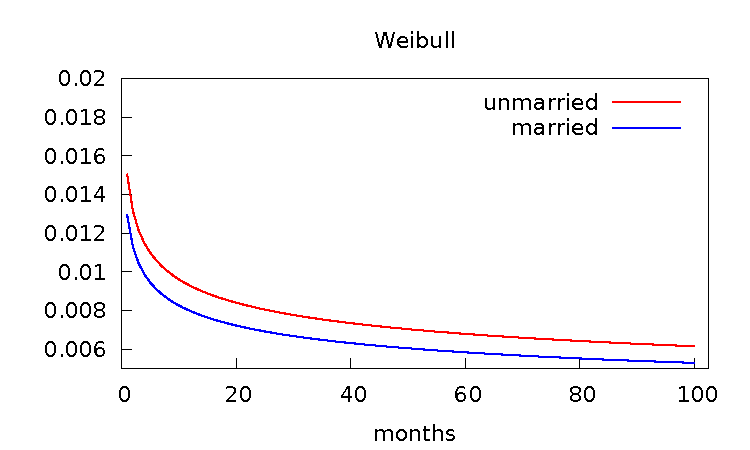
\includegraphics[scale=0.85]{figures/weibull}
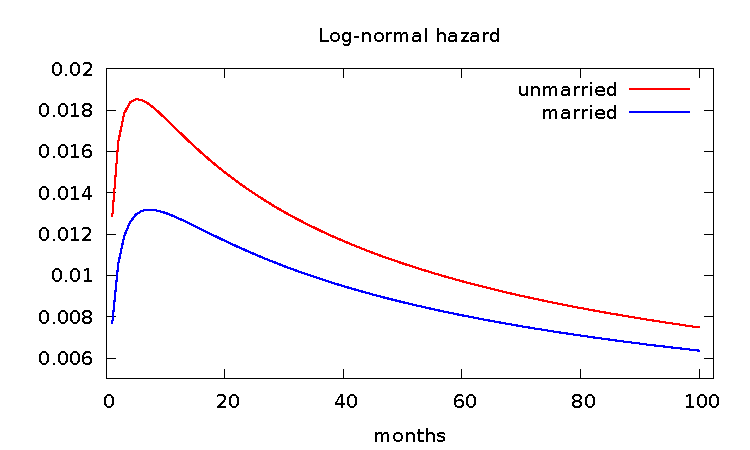
\includegraphics[scale=0.85]{figures/lognorm}
\caption{Recidivism hazard estimates for married and unmarried
  ex-convicts}
\label{fig:hazard-plots}
\end{figure}

\subsection{Alternative representations of the Weibull model}

One point to watch out for with the Weibull duration model is that the
estimates may be represented in different ways.  The representation
given by \app{gretl} is sometimes called the \textit{accelerated
  failure-time} (AFT) metric. An alternative that one sometimes sees
is the \textit{log relative-hazard} metric; in fact this is the metric
used in Wooldridge's presentation of the recidivism example.  To get
from AFT estimates to log relative-hazard form it is necessary to
multiply the coefficients by $-\sigma^{-1}$. For example, the
\texttt{married} coefficient in the Weibull specification as shown
here is 0.188104 and $\hat{\sigma}$ is 1.24090, so the alternative
value is $-0.152$, which is what Wooldridge shows
(\citeyear{wooldridge-panel}, Table 20.1).

\subsection{Fitted values and residuals}

By default, \app{gretl} computes fitted values (accessible via
\dollar{yhat}) as the conditional mean of duration.  The formulae
are shown below (where $\Gamma$ denotes the gamma function, and the
exponential variant is just Weibull with $\sigma = 1$).

\begin{center}
\setlength\tabcolsep{1em}
\begin{tabular}{ccc}
Weibull & Log-logistic & Log-normal \\ [4pt]
$\exp(X\beta)\Gamma(1 + \sigma)$ &
$\displaystyle \exp(X\beta)\frac{\pi \sigma}{\sin(\pi \sigma)}$ &
$\exp(X\beta + \sigma^2/2)$
\end{tabular}
\end{center}

The expression given for the log-logistic mean, however, is valid only
for $\sigma < 1$; otherwise the expectation is undefined, a point that
is not noted in all software.\footnote{The \texttt{predict} adjunct to
  the \texttt{streg} command in \app{Stata} 10, for example, gaily
  produces large negative values for the log-logistic mean in duration
  models with $\sigma > 1$.}

Alternatively, if the \verb|--medians| option is given, \app{gretl}'s
\texttt{duration} command will produce conditional medians as the
content of \dollar{yhat}.  For the Weibull the median is
$\exp(X\beta)(\log 2)^\sigma$; for the log-logistic and log-normal it
is just $\exp(X\beta)$.

The values we give for the accessor \dollar{uhat} are generalized
(Cox--Snell) residuals, computed as the integrated hazard function,
which equals the negative of the log of the survivor function:
\[
\hat{u}_i = \Lambda(t_i, x_i, \theta) = -\log S(t_i, x_i, \theta)
\]
Under the null of correct specification of the model these generalized
residuals should follow the unit exponential distribution, which has
mean and variance both equal to 1 and density $e^{-1}$. See
\cite{cameron-trivedi05} for further discussion.

%%% Local Variables: 
%%% mode: latex
%%% TeX-master: "gretl-guide"
%%% End: 
